\documentclass[a4paper,14pt,oneside,openany]{memoir}
\usepackage[utf8]{inputenc}
\usepackage[T1,T2A]{fontenc}
\usepackage[english, russian]{babel}                % Настройки для русского языка
\usepackage{times}
\usepackage{array}
\setlength{\arrayrulewidth}{0.005 mm}
\usepackage{xcolor}
\usepackage{lipsum}
\usepackage{ragged2e}

\usepackage[left=30mm, right=10mm, top=20 mm, bottom=20mm]{geometry}

\usepackage{multirow,makecell}                      % Улучшенное форматирование таблиц
\usepackage{booktabs}                               % Еще один пакет для красивых таблиц
\usepackage{soulutf8}                               % Поддержка переносоустойчивых подчёркиваний и зачёркиваний
\usepackage{icomma}                                 % Запятая в десятичных дробях
\usepackage{hyphenat}                               % Для красивых переносов
\usepackage{textcomp}                               % Поддержка "сложных" печатных символов типа значков иены, копирайта и т.д.
\usepackage[version=4]{mhchem}                      % Красивые химические уравнения
\usepackage{amsmath}                                % Усовершенствование отображения математических выражений 


\pagestyle{plain} % Убираем стандарные для данного класса верхние колонтитулы с заголовком текущей главы, оставляем только номер страницы снизу по центру

%%% Задаем параметры оглавления %%%

\usepackage{indentfirst} % Добавляем отступ к первому абзацу
\linespread{1} % Межстрочный интервал (наиболее близко к вордовскому полуторному) - тут вместо этого используется команда OnehalfSpacing*
\parindent=0.8cm % Абзацный отступ
\renewcommand*{\chapternumberline}[1]{} % Делаем так, чтобы номер главы не печатался
\renewcommand*{\cftchapterfont}{\normalfont\MakeUppercase} % Названия глав обычным шрифтом заглавными буквами
\addto\captionsrussian{\renewcommand\contentsname{Содержание}} % Меняем слово "Оглавление" на "Содержание"
\setrmarg{2.55em plus1fil} % Запрещаем переносы слов в оглавлении

\renewcommand*{\cftchapternumwidth}{1.5em} % Ставим подходящий по размеру разделитель между номером главы и самим заголовком
\setsecnumdepth{subsection} % Номера разделов считать до третьего уровня включительно, т.е. нумеруются только главы, секции, подсекции
\renewcommand*{\chapterheadstart}{} % Переопределяем команду, задающую отступ над заголовком, чтобы отступа не было
\renewcommand*{\printchapternum}{} % То же самое для номера главы
\renewcommand*{\printchaptername}{} % Переопределяем команду, печатающую слово "Глава", чтобы оно не печалось
\renewcommand*{\cftchapterfont}{\normalfont\textbf\MakeUppercase} % Названия глав обычным шрифтом заглавными буквами
\renewcommand*{\cftchapterpagefont}{\normalfont} % Номера страниц обычным шрифтом
\renewcommand*{\cftchapterleader}{\cftdotfill{\cftchapterdotsep}} % Делаем точки стандартной формы (по умолчанию они "жирные")
\renewcommand*{\cftchapterdotsep}{\cftdotsep} % Делаем точки до номера страницы после названий глав
\renewcommand*{\cftdotsep}{1} % Задаем расстояние между точками
\renewcommand*{\chapnumfont}{\normalfont\bfseries} % Меняем стиль шрифта для номера главы: нормальный размер, полужирный
\renewcommand*{\afterchapternum}{\hspace{1em}} % Меняем разделитель между номером главы и названием
\renewcommand*{\printchaptertitle}{\normalfont\bfseries\centering\MakeUppercase} % Меняем стиль написания для заголовка главы: нормальный размер, полужирный, центрированный, заглавными буквами
\setbeforesecskip{10pt} % Задаем отступ перед заголовком секции
\setaftersecskip{10pt} % Ставим такой же отступ после заголовка секции
\setsecheadstyle{\raggedright\normalfont\bfseries} % Меняем стиль написания для заголовка секции: выравнивание по правому краю без переносов, нормальный размер, полужирный
\renewcommand*{\printchapternum}{} 

\maxtocdepth{subsection} % В оглавление попадают только разделы первыхтрех уровней: главы, секции и подсекции

%%% Выравнивание и переносы %%%

\tolerance 1414
\hbadness 1414
\emergencystretch 1.5em                             % В случае проблем регулировать в первую очередь
\hfuzz 0.3pt
\vfuzz \hfuzz
%\dbottom
%\sloppy                                            % Избавляемся от переполнений
\clubpenalty=10000                                  % Запрещаем разрыв страницы после первой строки абзаца
\widowpenalty=10000                                 % Запрещаем разрыв страницы после последней строки абзаца
\brokenpenalty=4991                                 % Ограничение на разрыв страницы, если строка заканчивается переносом


%%% Настраиваем отображение списков %%%

\usepackage{enumitem}                               % Подгружаем пакет для гибкой настройки списков
\makeatletter
    \AddEnumerateCounter{\asbuk}{\russian@alph}     % Объясняем пакету enumitem, как использовать asbuk
\makeatother
\renewcommand{\labelenumii}{\asbuk{enumii}}        % Кириллица для второго уровня нумерации
\renewcommand{\labelenumiii}{\arabic{enumiii}}     % Арабские цифры для третьего уровня нумерации
\setlist{noitemsep, leftmargin=*}                   % Убираем интервалы между пунками одного уровня в списке
\setlist[1]{labelindent=\parindent}                 % Отступ у пунктов списка равен абзацному отступу
\setlist[2]{leftmargin=\parindent}                  % Плюс еще один такой же отступ для следующего уровня
\setlist[3]{leftmargin=\parindent}                  % И еще один для третьего уровня

%%% Счетчики для нумерации объектов %%%

\counterwithout{equation}{chapter}                  % Сквозная нумерация математических выражений по документу
%\counterwithout{table}{chapter}   


%%% Задаем параметры оформления рисунков и таблиц %%%

\usepackage{graphicx, caption, subcaption} % Подгружаем пакеты для работы с графикой и настройки подписей
\graphicspath{{images/}} % Определяем папку с рисунками
\captionsetup[subfigure]{font=small, width=\textwidth, name=Рис., justification=centering} 
\captionsetup[table]{singlelinecheck=false,font=small,width=\textwidth,justification=justified} % Задаем параметры подписей к таблицам: запрещаем переносы, маленький шрифт (в данном случае 12pt), ширина равна ширине текста, выравнивание по ширине
\captiondelim{ --- } % Разделителем между номером рисунка/таблицы и текстом в подписи является длинное тире
\setkeys{Gin}{width=\textwidth} % По умолчанию размер всех добавляемых рисунков будет 
\usepackage[section]{placeins} % Объекты типа float (рисунки/таблицы) не вылезают за границы секциии, в которой они объявлены
% Зачем: Включение номера раздела в номер рисунка. Нумерация рисунков внутри раздела.


\usepackage{caption}
\usepackage{subcaption}
\captionsetup[subfigure]{labelformat=empty} 
%%% Вставляем по очереди все содержательные части документа %%%
\begin{document}

\thispagestyle{empty}

\begin{center}
    Учреждение образования \\
"<Брестский государственный университет имени А. С. Пушкина"> \\
Физико-математический факультет \\
Кафедра общей и теоретической физики \\


    \vspace{20pt}
\end{center}

\begin{flushright}
    \begin{minipage}{0.4\textwidth}
      К защите допустить:\\[0.8em]
      Заведующий кафедрой \\[0.45em]
      \underline{\hspace*{2.8cm}}~Демидчик А.\,В.
    \end{minipage}\\[2.2em]
    
  \end{flushright}

\vspace{50pt}
  \begin{center}
    \textbf{Дипломная работа} \\  
    \vspace{20pt}
  Компьютерное моделирование молекулярно-кинетических процессов
  
\end{center}
\vfill
    \vspace{20 pt}
\noindent{
  Выполнила студентка 4 курса гр. КФ-41 \hrulefill \: Я.\,С.~Ситковец 
    }


\vspace{20 pt}
 \noindent
 \begin{tabular}{lp{4em}l}
   Научный руководитель:   &&  Доктор физико-математических наук, \\ \\
                          &&   профессор \hrulefill  ~Плетюхов В.\,А
 \end{tabular}
 \vfill
  
 \begin{center}
    {\normalsize Брест 2023}
  \end{center}
      % ТИТУЛЬНЫЙ ЛИСТ
\newpage             % Переходим на новую страницу
\setcounter{page}{2} % Начинаем считать номера страниц со второй
%\OnehalfSpacing* % Задаем полуторный интервал текста (в титульнике одинарный, поэтому команда стоит после него)
\tableofcontents*    % Автособираемое оглавление

\chapter*{ВВЕДЕНИЕ}
\addcontentsline{toc}{chapter}{Введение}
\label{ch:intro}
Местом прохождения практики был выбран отдел программирования ОАО «Савушкин продукт» с 23.01.2023 г. по 13.05.2023 г.
Цель практики: ознакомиться с деятельностью предприятия, получить практический опыт работы и навыки для написания дипломной работы.
Задачи практики:
\begin{itemize}
        \item Сбор материала для дипломной работы по теме «Компьютерное моделирование молекулярно-кинетических процессов».Получения практического опыта работы с контроллерами и аналоговыми устройствами, в частности с датчиком температуры.
        \item  Изучение различных библиотечных функций С++ и Python для математичесикх расчетов и визуализации данных.
        \item Ознакомиться с рабочим процессом отдела программирования.
        \item Оформление дипломной работы на GitHub c помощью языков разметки Markdown и \LaTeX .
    \end{itemize}

\endinput
    % ВВЕДЕНИЕ
\chapter{ГЛАВА 1. ОПИСАНИЕ МОДЕЛИРУЕМЫХ ФИЗИЧЕСКИХ ЯВЛЕНИЙ}
\label{ch:chapter1}

\section{Распределение Максвелла-Больцмана}
Если система находится в состоянии равновесия, то средние значения любых ее параметров не будут зависеть от времени. Поэтому функция распределения должна зависеть только от интегралов движения системы. Основным интегралом движения является полная механическая энергия системы $E$ или функция Гамильтона $H$. Соответсвенно простейший общий вид функции распределения будет $w(x)=w(H)$. Конкретный же вид этой функции $w(H)$ нужно определить. Функция Гамильтона зависит от $6N$ переменных системы $x$ и от внешних параметров $a$, т. е. $H(x,a)$. [1]

Для идеального газа функцию  Гамильтона $H(x,a)$ можно просто заменить энергией $E(x)$, тогда по формуле канонического распределения Гиббса для изотермической системы

$$w(x)=e^{\frac{\psi - H(x, a)}{\theta}} \quad (1.1.1)$$

вероятность нахождения системы с энергией $E$ в элементе фазового пространства $(dx)^{6N}$ будет
$$dW(x)=e^{\frac{\psi - E}{\theta}}=const \: e^{-\frac{E}{kT}}(dx)^{6N}. \quad (1.1.2)$$

Для системы невзаимодействующих частиц энергию $E$ можно представить как сумму энергий отдельных частиц $E=\sum_{i=1}^{N} E_i$. Тогда вероятность (1.1.1) можно разбить на $N$ сомножителей

$$dW(x)=const \: e^{-\frac{E_i}{kT}}dx_1dy_1dz_1dp_{x_1}dp_{y_1}dp_{z_1}...$$

$$...e^{-\frac{E_N}{kT}}dx_Ndy_Ndz_Ndp_{x_N}dp_{y_N}dp_{z_N}. \quad (1.1.3)$$

Интегрируя по $6(N-1)$ переменной всех частиц, кроме $i$-й, получим выражение вероятностей для $i$-й частицы:

$$dW(x_i,y_i,z_ip_{xi}p_{yi}p_{zi})=const \: e^{-\frac{E_i}{kT}}dx_idy_idz_idp_{x_i}dp_{y_i}dp_{z_i} \quad (1.1.4)$$

Здесь $E_i$ рассматривается как функция $6$ переменных $p_{x_i}$, $p_{y_i}$, $p_{z_i}$, $x_i$, $y_i$, $z_i$. Распределение (1.2.4) можно рассматривать в $6$-мерном фазовом пространстве одной молекулы, которое называют $\mu$-пространством ($\mu$ $-$ от слова молекула). [1]

Энергия отдельной частицы $E_i$ может быть представлена суммой кинетической и потенциальной энергий, зависящих от импульса и координат частицы, соответственно:

$$E=E_\text{кин}+E_{\text{пот}}=\frac{p_{x}^2+p_{y}^2+p_{z}^2}{2m}+ U(x,y,z)\quad (1.1.5)$$

Подставляя это выражение в (1.1.4), получим

$$dW(p_x,p_y,p_z, x,y,z)=const \: e^{-\frac{\frac{p_{x}^2+p_{y}^2+p_{z}^2}{2m}+ U(x,y,z)}{kT}}dp_xdp_ydp_zdxdydz. \quad (1.1.6)$$

Это и есть распределение Максвелла-Больцмана.

Тот факт, что кинетическая и потенциальная энергии зависят от разных переменных, дает возможность рассмотреть одно распределение (1.1.6) как два независимых распределения в трехмерном пространстве импульсов и в трехмерном пространстве координат:

$$dW(p_x,p_y,p_z)=Ae^{-\frac{p_{x}^2+p_{y}^2+p_{z}^2}{2mkT}}dp_xdp_ydp_z, \quad (1.1.7)$$

$$dW(x,y,z)=Be^{-\frac{U(x,y,z)}{kT}}dxdydz. \quad (1.1.8)$$

Здесь $A$ и $B$ $—$ постоянные, определяемые из условия нормировки распределений.

Функция распределения по координатам частицы (1.1.8) в потенциальном поле представляет так называемое распределение Больцмана (1877 г.). [1]

$$dW(z)=Be^{-\frac{U(z)}{kT}}dz. \quad (1.1.9)$$

Для идеального газа в однородном поле силы тяжести из (1.1.9) выводится известная барометрическая формула. Действительно, в этом случае $U(z)=mgz$ и функция распределения частиц по высоте $z=h$ принимает вид

$$f(z)=\frac{dW(z)}{dz}=Be^{-\frac{mgz}{kT}}. \quad (1.1.10)$$

Вследствие пропорциональности числа частиц $n(z)$ функции распределения (1.1.10) получим следующее распределение числа частиц в единице объема по высоте $z$:

$$n(z)=const \: e^{-\frac{mgz}{kT}}.$$

Поскольку при $z=0$ в единице объема будет $n_0$ частиц, то для распределения частиц по высоте получим

$$n(z)= n_0 e^{-\frac{mgz}{kT}}. \quad (1.1.11)$$

Если учесть, что в газе давление пропорционально плотности, то из (1.1.11) получается барометрическая формула

$$\rho(z)= \rho_0 e^{-\frac{mgz}{kT}}. \quad (1.1.12)$$

Экспериментальные исследования показали, что на больших высотах в атмосфере наблюдаются отклонения числа частиц от распределения, описываемого формулой (1.1.11), связанные с неоднородным составом атмосферы, с различием температур на разных высотах и с тем, что атмосфера не находится в состоянии равновесия.
В атмосферах планет происходит явление рассеяния атмосферы в космическое пространство. Оно объясняется тем, что всякая частица, имеющая скорость больше второй космической для данной планеты, может покинуть атмосферу планеты. В газе, как следует из максвелловского распределения, всегда имеется некоторая доля молекул с очень большими скоростями, уход которых и определяет постепенное рассеяние верхних слоев атмосферы. Рассеяние атмосферы планет происходит тем быстрее, чем меньше масса планеты и выше ее температура. [1]

Для Земли этот эффект оказывается ничтожно малым, а планета Меркурий и Луна уже потеряли таким способом свои атмосферы.

\section{Распределение Максвелла}

Рассмотрим поступательное движение частиц максвелл-больцмановского идеального газа, пренебрегая квантованием энергии. Из формул распределения Максвелла-Больцмана

$$dN=e^{(\mu - \epsilon)/kT} \frac{dГ}{h^f}, \quad (1.2.1)$$

$$N=\int e^{(\mu - \epsilon)/kT} \,\frac{dГ}{h^f} \quad (1.2.2)$$

получаем выражение для вероятности нахождения изображающей точки в элементе объема $d\text{Г}$-пространства

$$ dW=\frac{dN}{N}=\frac{e^{- \epsilon/kT}d\text{Г}}{\int e^{- \epsilon/kT}\,dГ}, \quad (1.2.3)$$

где выражение, стоящее в знаменателе, есть статистический интеграл $Z$. [2] Мы будем рассматривать газ, состоящий нз молекул с произвольным числом $n$ атомов в молекуле. Поскольку, однако, нас интересует сейчас только поступательное движение, мы выделим из всех обобщенных координат и импульсов молекулы три координаты центра масс $(x, y, z)$ и соответствующие им проекции полного импульса молекулы $(\xi,\eta, \zeta)$, и представим энергию молекулы в виде

$$\epsilon = \frac{\rho^2}{2m}+U(x,y,z)+\epsilon' \quad (1.2.4)$$

где $\rho^2=\xi^2 + \eta^2 + \zeta^2$ $-$ квадрат импульса молекулы как целого, $U(x, y, z)$ $-$ потенциальная энергия молекулы во внешнем поле (предполагается, что она не зависит от ориентации молекулы) и $\epsilon'$ $-$ энергия остальных степеней свободы, не зависящая от $(x, y, z,\xi,\eta, \zeta)$. Интегрируя выражение (1.2.3) по всем степеням свободы кроме поступательных, мы найдем вероятность того, что центр масс молекулы лежит в объеме $dV$, а импульс ее заключен в интервале $(\rho, \rho +d \rho)$. Эта вероятность распадается на два сомножителя: один зависит только от импульса, а другой $-$ только от координат

$$ dW= \frac{e^{- \rho^2/2mkT}dV_\rho}{\int e^{- \rho^2/2mkT}\, dV_\rho} \frac{e^{- U(x,y,z)/kT}dV}{\int e^{- U(x,y,z)/kT}\, dV}.\quad (1.2.5)$$

Это значит, что распределение молекул по импульсам и распределение их по координатам не зависят друг от друга. Интегрируя выражение (1.2.5) по координатам, получим

$$ dW(\rho)= \frac{e^{- \rho^2/2mkT}dV_\rho}{\int e^{- \rho^2/2mkT}\, dV_\rho}.\quad (1.2.6)$$

Записав элемент объема пространства импульсов в виде $dV_p = 4\pi\rho^2d\rho$ и вычисляя интеграл, стоящий в знаменателе

$$4\pi \int_{0}^{\infty} e^{-\frac{\rho^2}{2mkT}}\rho^2\, d\rho = 4\pi J_2 =(2\pi mkT)^{3/2},$$

получим распределение молекул газа по импульсам

$$ dW(\rho)= \frac{4\pi}{(2\pi mkT)^{3/2}} e^{-\frac{\rho^2}{2mkT}}\rho^2 d\rho.\quad (1.2.7)$$

Переходя от импульса к скорости, имеем

$$ dW(v)= 4\pi \left(\frac{m}{2\pi kT}\right)^{3/2} e^{-\frac{mv^2}{2kT}}v^2 dv.\quad (1.2.8)$$

Формулы (1.2.7), (1.2.8) называются формулами распределения Максвелла и позволяют решать ряд конкретных задач. [2]

Найдем наиболее вероятную скорость молекул газа. Для этой скорости выражение (1.2.8) должно иметь максимум:

$$\frac{d}{dv}\left(v^2e^{-\frac{mv^2}{2kT}}\right)=ve^{-\frac{mv^2}{2kT}}\left( 2 - \frac{mv^2}{kT}\right)=0,$$

откуда

$$v_\text{в}=\sqrt{\frac{2kT}{m}}.\quad (1.2.9)$$

Легко также найти среднюю и среднюю квадратичную скорость молекул

$$v=\int v\,dW(v)=4\pi \left(\frac{m}{2\pi kT}\right)^{3/2}\int_{0}^{\infty}v^3e^{-\frac{mv^2}{2kT}}\, dv= \sqrt{\frac{8kT}{\pi m}},\quad (1.2.10)$$

$$\overline{v^2}=\int v^2\,dW(v)=4\pi \left(\frac{m}{2\pi kT}\right)^{3/2}\int_{0}^{\infty}v^4e^{-\frac{mv^2}{2kT}}\, dv= \frac{3kT}{ m}.\quad (1.2.11)$$

Отсюда средняя энергия поступательного движения молекул равна

$$\overline{E_\text{к}}=\frac{m\overline{v^2}}{2}=\frac{3}{2}kT.$$

График распределения Максвелла имеет вид, изображенный на рис. 1.2.1. С повышением температуры максимум кривой смещается
\begin{figure}[ht]
	\centering
\hspace*{\fill}%
\begin{subfigure}[b]{0.49\textwidth}
        \centering
		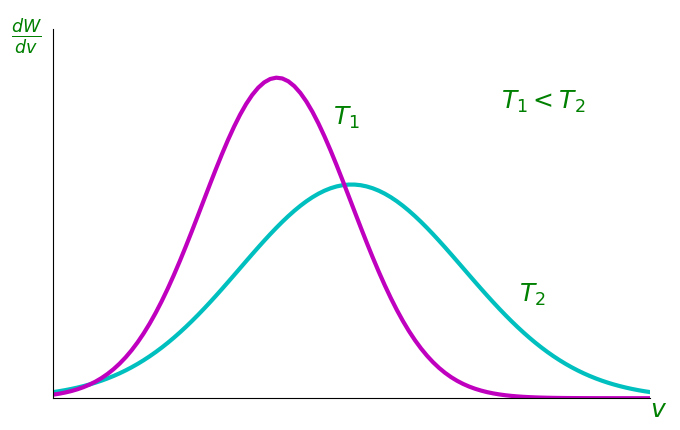
\includegraphics[height=5cm,keepaspectratio]{images/maxwell2.png}
        \caption{Рис. 1.2.1}
	\end{subfigure}
	\begin{subfigure}[b]{0.49\textwidth}
        \centering
		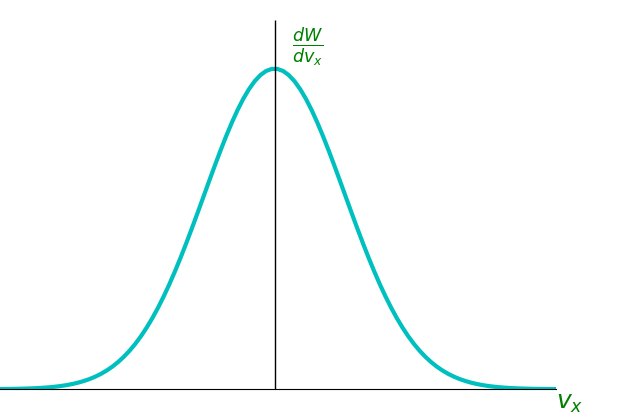
\includegraphics[height=5cm,keepaspectratio]{images/maxwell1.png}
		\caption{Рис. 1.2.2}
	\end{subfigure}
 \hfill
 \hspace*{\fill}%
 \end{figure}

 в сторону высоких температур и сам график становится более пологим с более существенным «хвостом», тянущимся в область больших скоростей.

Если рассекать импульсное пространство не на шаровые слои, а на параллелепипеды $dv_x$, $dv_y$, $dv_z$, то распределение (1.2.6) можно записать в виде произведения трех множителей вида

$$dW(v_i)=\left( \frac{m}{2 \pi kT}\right)^{1/2}e^{-\frac{mv_i^2}{2kT}}dv_i\quad (i=x,y,z). \quad (1.2.12)$$

Это свидетельствует о том, что распределения по величине разных проекций скорости независимы. График распределения Максвелла по проекциям скорости имеет вид, изображенный на рис. 1.2.2.

Нетрудно понять из физических соображений и проверить путем прямого вычисления, что среднее значение проекций $v_x$, $v_y$, $v_z$ равно нулю. Сделаем в заключение следующее замечание. Хотя мы вывели распределение Максвелла для идеального газа, оно на самом деле имеет значительно более широкую область применимости. Оно справедливо для всех систем взаимодействующих частиц, если температура настолько высока, что можно пренебрегать квантованием энергии. Это следует из того, что распределение Максвелла может быть получено из канонического распределения Гиббса, если представить энергию системы в виде $E = mv_i^2/2 + E'$, где $E'$ $-$ энергия системы (включая и энергию взаимодействия молекул) за вычетом кинетической энергии центра инерции $i$-й молекулы, и проинтегрировать функцию распределения по координатам всех молекул и по всем обобщенным скоростям, кроме скорости центра инерции $i$-й молекулы. [2]

\section{Броуновское движение}

Молекулярное движение приводит к диффузии, к проникновению молекул одного газа в другой.

Пусть вдоль оси $Oz$ имется градиент концетрации некоторого примесного газа в основном газе. Тогда через едничную площадку в единицу времени снизу перемещается больше молекул диффундирующего газа, а сверху (где концетрация ниже) $-$ меньше. Таким образом, возникает направленный поток газа снизу вверх. Поток газа, вызванный диффузией, удовлетворяет закону Фика
$$ I = D\frac{dc}{dz}, \quad (1.3.1)$$

где $D$ $-$ коэффициент диффузии. [1]

Для вычисления этого коэффициента рассмотрим диффузионный поток газа. Снизу вверх в слой $z$ через единичную площадку за время $dt$  проходит $\frac{\overline{v}n_1dtS}{6}$ молекул диффундирующего газа, а сверху из слоя $z+l$ вниз $- \frac{\overline{v}n_2dtS}{6}$ молекул.

Из самого слоя $z$ в слои $z+l$ и $z-l$ уходит $\frac{\overline{v}n_0dtS}{3}$ молекул. Разность этих велечин дает число молекул, перемещающихся за время $dt$ через площадку $S$ в направлении от слоя $z-l$ к слою $z+l$;
$$dn = \frac{\overline{v}Sdt}{6}(n_2+n_1-2n_0).$$

Здесь $n_1$, $n_0$ и $n_2 -$ среднее число молекул в слоях $z+l$, $z$ и $z-l$, отстоящих друг от друга на расстоянии $l$ и отличающихся по числу молекул на $\Delta n = \frac{dc}{dz}l$.

Поток частиц от слоя с большей концетрацией к слою с меньшей концетрацией равен
$$l=\frac{\Delta n}{S \Delta t}= \frac{\overline{v}S\Delta t}{6S \Delta t} \cdot 2 \cdot \frac{dc}{dz}l= \frac{\overline{v}l}{3} \frac{dc}{dz}. \quad (1.3.2)$$

А следовательно коэффициент диффузии определится соотношением
$$D=\frac{l}{\frac{dc}{dz}}= \frac{\overline{v}l}{3}. \quad (1.3.3)$$

Здесь $\overline{v}$ $-$ средняя скорость молекул, считается независящей от концетрации и $l$ $-$ средняя длина свободного пробега. Коэффициент диффузии, таким образом, оказывается $\overline{v}$ и от давления или плотности газа через $l$. [1]

Эта формула для коэффициента диффузии с учетом выражения длины свободного пробега часто используется для оценки эффективного диаметра (размеров) молекул $d_0$.

Броуновское движение $-$ непрерывное, беспорядочное движение малых частиц, взвешенных в жидкости или газе, происходящее под действием ударов молекул окружающей среды. Броуновское движение представляет собой одно из наиболее ярких и доступных наблюдению проявлений молекулярно-кинетической природы хаотического теплового движения атомов и молекул.
Причина броуновского движения — тепловое движение молекул среды и отсутствие точной компенсации ударов, испытываемых частицей со стороны окружающих её молекул, т. е. броуновское движение обусловлено флуктуациями давления (флуктуации — это случайные отклонения физических величин от их средних значений). Эти флуктуации в числе ударов $\Delta n$ по статистическим законам пропорциональны $\frac{1}{\sqrt{n}}$. Поэтому, если частица большая, т. е. с ней сталкивается одновременно большое число молекул $n$, то флуктуации $\Delta n$ будут очень малы и большая частица не придет в движение. Если частица имеет микроскопические размеры, то число столкновений $n$ будет невелико, а флуктуации $\Delta n$ большие. Благодаря флуктуациям происходит необратимое перемещение броуновкой частицы.

Хотя броуновская частица движется в результате хаотических столкновений с молекулами среды и невозможно точно определить ее траекторию, статистические методы позволяют определить среднее квадратичное отклонение частицы от начального положения как функцию времени. Найдем закон движения броуновской частицы в среде с коэффициентом вязкости $\eta$.

Уравнение движения броуновской частицы имеет вид
$$M\ddot{r} = R(t) - 6 \pi \eta ar. \quad (1.3.4)$$

Здесь $M -$ масса частицы, $r -$ ее радиус-вектор, $6\pi \eta ar -$ вязкая сила, действующая на частицу, имеющую скорость $r$ и радиус $a$, и наконец $R(t) -$ мгновенная равнодействующая всех сил ударов молекул о частицу. Умножим уравнение (1.3.4) скалярно на $r$:
$$M(\ddot{r}r)= rR(t)- 6\pi \eta a(\dot{r} r) \quad (1.3.5) $$

и воспользовавшись вспомогательными соотношениями

$$(\dot{r}r)=\frac{1}{2} \cdot \frac{d^2}{dt^2}(r^2)- r^2, $$

перепишем уравнение (1.3.5) в виде
$$ M \frac{d^2}{dt^2}\left(\frac{r^2}{2}\right) + 6 \pi \eta a \frac{d}{dt}\left( \frac{r^2}{2}\right) = M\dot{r}^2 + rR(t).$$

Проинтегрируем последнее уравнение один раз по времени и разделим почленно на t:

$$\frac{M}{t} \cdot \frac{d}{dt}\left(\frac{r^2}{2}\right) + \frac{6 \pi }{t} \eta a\left( \frac{r^2}{2}\right)=\frac{1}{t} \int_{0}^{1}Mr^2\,dt + \frac{1}{t}\int_{0}^{1}rR(t)\,dt. \quad (1.3.6)$$

Найдем значения выражений, стоящих в правой части. Первый член представляет удвоенную среднюю кинетическую энергию частицы за промежуток времени от $0$ до $t$. Так как благодаря столкновениям молекулы среды и броуновская частица непрерывно обмениваются энергией, то на одну степень свободы частицы в среднем приходится энергия $\frac{kT}{2}$. Поскольку в поле микроскопа мы рассматриваем движение частицы в плоскости, т. е. с двумя степенями свободы, то кинетическая энергия плоского движения будет равна $kT$, т. е.
$$\frac{1}{t} \int_{0}^{1} M\dot{r}^2 \, dt = 2kT.$$

Второй член есть среднее значение произведения $r(t)R(t)$ за тот же интервал времени. Вследствие хаотичности движения частицы и действующих на частицу сил оно равно нулю:

$$ \frac{1}{t}\int_{0}^{1}r(t)R(t) \, dt = 0.$$

Поэтому уравнение (1.3.6) можно переписать так:

$$\frac{M}{t}\frac{d}{dt}\left(\frac{r^2}{2}\right) + \frac{6\pi a\eta}{t}\left(\frac{r^2}{2}\right) =2kT. \quad (1.3.7)$$

Вводя переменную $z=r^2$, получаем линейное уравнение

$$M\dot{z} + 6 \pi a \eta z = 4kTt, \quad (1.3.8) $$

решением которого является сумма общего решения однородного уравнения и частное решение неоднородного. Решение однородного уравнения имееет вид:

$$z_{\text{одн}} = Ce^{-\frac{6\pi a \eta t}{M}} \quad (1.3.9)$$

и для больших интервалов времени обращается в нуль. Частное решение неоднородного уравнения ищем в виде

$$z_{\text{неодн}}=At.$$

Подставляя его в (1.3.8), получаем выражение для $A$:
$$A = \frac{4kTt}{6\pi \eta t + M} .$$

Пренебрегая в знаменателе массой $M$, для больших промежутков времени ($t  \rightarrow \infty$) получим

$$z_{\text{неодн}}=\frac{4kT}{6 \pi a \eta}t=\frac{2kTt}{3 \pi a \eta}. \quad (1.3.10)$$

Таким образом, решением уравнения движения броуновской частицы за большие промежутки времени, когда $r^2$ можно считать за средний квадрат смещения частицы в плоскости $\overline{r^2}$, будет выражение

$$r^2 = \overline{r^2}=2\frac{kT}{3 \pi a \eta}t. \quad (1.3.11)
$$

Формула (1.3.11) называется формулой Эйнштейна-Смолуховского. Она показывает, что среднее квадратичное смещение броуновской частицы $\sqrt{\overline{r^2}}$ зависит от температуры и вязкости среды, размеров частиц и пропорционально корню квадратному из времени наблюдения.

Далее, заменяя $\frac{kT}{3 \pi a \eta}$ коэффициентом диффузии $D$, для среднего квадрата смещения $\overline{r^2}$ броуновской частицы за время $t$  получаем выражение

$$\overline{r^2}=2Dt. \quad (1.3.12)$$

Смещения отдельных броуновских частиц в плоскости от начального положения являются случайными величинами и будут распределяться около среднего квадратичного смещения по гауссовскому закону. Вероятность того, что частица за время $t$ сместится на расстояние $x$ от начального положения равна

$$dW(x)=Ae^{-\frac{x^2}{2\overline{r^2}}}dx.$$

По аналогии запишем
$$dW(y)=Ae^{\frac{y^2}{2\overline{r^2}}}dy.$$

Вероятность смещения в плоскости на расстояние $r$

$$dW(r)=A^2e^{-\frac{x^2}{2r^2}}dy=2 \pi A^2e^{-\frac{r^2}{2\overline{r^2}}}rdr. \quad (1.3.13)$$

Последняя формула хорошо удовлетворяется на опыте.

\chapter{ГЛАВА 2. ИСПОЛЬЗУЕМЫЕ МОДУЛИ}
\label{ch:chapter2}

\section{Компьютерное моделирование и языки программирования}

Одним из наиболее распространенных языков программирования для моделирования является MATLAB. Этот язык используется для решения математических задач, анализа данных и создания графиков. MATLAB имеет большое количество встроенных функций и инструментов для работы с матрицами и векторами, что делает его очень удобным для создания математических моделей.

Другим популярным языком программирования для компьютерного моделирования является Python. Python $-$ это интерпретируемый язык программирования, который используется для разработки программного обеспечения, анализа данных и машинного обучения. Он имеет простой и понятный синтаксис, что делает его доступным для начинающих программистов. Также можно выделить C++, C\#, Java, JavaScript и др. Каждый из этих языков имеет свои преимущества и недостатки в зависимости от задачи, которую нужно решить.

Кроме языков программирования, для компьютерного моделирования используются специализированные программные средства, такие как Simulink, ANSYS, COMSOL и др. Эти программы предоставляют готовые блоки для создания математических моделей и имеют широкий набор инструментов для анализа результатов моделирования.

\section{JavaScript и Canvas}

JavaScript $-$ это язык программирования, который широко используется для создания интерактивных веб-страниц. Одним из самых популярных приложений JavaScript является создание графики и анимации в вебе с использованием технологии Canvas.

Canvas $-$ это мощный элемент HTML5, который позволяет разработчикам создавать динамическую, интерактивную графику на веб-страницах. С помощью Canvas можно рисовать фигуры, линии, текст и изображения, а также анимировать их в реальном времени. Это делает его идеальным инструментом для создания игр, диаграмм, визуализаций данных и других интерактивных веб-приложений.

Одним из ключевых преимуществ использования Canvas с JavaScript является то, что он позволяет быстро и плавно отображать графику, даже на мобильных устройствах. Это происходит потому, что Canvas использует аппаратное ускорение для рендеринга графики, что означает, что он использует GPU (графический процессор) устройства для выполнения вычислений и быстрого рисования графики.

\section{Python и модули для визуализации данных}

Для написания программ используются Python 3.11.2 с пакетами Pygame, Pymunk, Random, Matplotlib и Numpy.

Python $-$ высокоуровневый язык программирования общего назначения с динамической строгой типизацией и автоматическим управлением памятью, ориентированный на повышение производительности разработчика, читаемости кода и его качества, а также на обеспечение переносимости написанных на нём программ. Язык является полностью объектно-ориентированным в том плане, что всё является объектами. [6]

Pygame — набор модулей (библиотек) языка программирования Python, предназначенный для написания компьютерных игр и мультимедиа-приложений. Pygame базируется на мультимедийной библиотеке SDL. [7]

Pymunk — это физический движок для языка программирования Python, который позволяет создавать физические симуляции, такие как игры или моделирование движения объектов. Он предоставляет различные функции для работы с твердыми телами, силами, столкновениями и т.д. [8]

Random $-$ это модуль языка программирования Python, который предоставляет функции для генерации случайных чисел. Он может использоваться для создания случайных чисел, выборки случайных элементов из списка, перемешивания списка и т.д. Python random использует различные алгоритмы для генерации чисел, включая алгоритм Mersenne Twister. [6]

Matplotlib $-$ это библиотека для языка программирования Python, которая предоставляет широкие возможности для создания различных графиков и визуализации данных. Она позволяет создавать различные типы графиков, включая линейные, столбчатые, круговые, гистограммы, диаграммы рассеяния и многое другое. Matplotlib также предоставляет возможности для настройки внешнего вида графиков, включая цвета, шрифты, размеры и т.д. Библиотека Matplotlib является одной из наиболее популярных библиотек для визуализации данных в Python. [9]

NumPy (Numerical Python) $-$ это библиотека для языка программирования Python, которая предоставляет поддержку для работы с многомерными массивами и матрицами, а также функции для выполнения математических операций над ними. NumPy является одним из основных инструментов для научных вычислений в Python и используется в таких областях, как машинное обучение, обработка изображений, анализ данных и других. NumPy также предоставляет множество функций для работы с линейной алгеброй, случайными числами, преобразованиями Фурье и другими математическими операциями. [10]

Для моделирования частиц в программе используется matplotlib.patches.

matplotlib.patches $-$ это модуль библиотеки Matplotlib для создания графических объектов (патчей) на графике. Он содержит классы для создания различных типов патчей, таких как прямоугольники, круги, многоугольники и т.д. [9]

Класс ParticlePatch в модуле matplotlib.patches используется для создания патчей, представляющих частицы в системах. Он позволяет задавать различные параметры частиц, такие как размер, цвет и положение на графике.

ParticlePatch может быть полезен в различных областях, таких как физика, химия и материаловедение, где важно визуализировать системы частиц и их поведение на графике.
\input{5_chapter3}
\chapter*{ЗАКЛЮЧЕНИЕ}
\addcontentsline{toc}{chapter}{ЗАКЛЮЧЕНИЕ}

В заключение можно сказать, что создание компьютерной модели является важным инструментом для исследования различных физических явлений. В данном дипломном проекте были рассмотрены три симуляции: броуновское движение, распределение молекул по скоростям и распределение частиц в поле тяжести.

Броуновское движение является одним из наиболее изученных явлений в физике. С помощью компьютерной модели удалось продемонстрировать, как частицы движутся в случайном порядке, что позволяет лучше понять механизмы этого явления.

Распределение молекул по скоростям является важным параметром в химии и физике. С помощью компьютерной модели удалось проанализировать, как изменяется распределение молекул при изменении температуры и других параметров.

Распределение частиц в поле тяжести также является важным явлением в физике. С помощью компьютерной модели удалось продемонстрировать, как частицы распределяются в поле тяжести, что позволяет лучше понять механизмы этого явления.

Таким образом, создание компьютерной модели является важным инструментом для исследования различных физических явлений. Разработанные симуляции позволяют лучше понимать механизмы броуновского движения, распределения молекул по скоростям и распределения частиц в поле тяжести.

\end{document}

